\chapter{Evaluation and Analysis}
\label{ch:evaluation}

This chapter details the methodology used to evaluate the Wolverine prototype \cite{christen2012data}. Crucially, it establishes an explicit evidence hierarchy to distinguish between verified functional behavior, theoretically bounded algorithms, and static evaluation mocks. It provides a forensic accounting of existing metric artifacts and outlines the rigorous methodology required for future dynamic benchmarking.

\section{Evaluation Philosophy}
\label{sec:eval-philosophy}
The Wolverine system cannot be evaluated using a single scalar accuracy metric because it spans fundamentally disparate domains. The evaluation is therefore separated into distinct dimensions:
\begin{itemize}
    \item \textbf{Functional Correctness:} Does the pipeline parse and project data without crashing?
    \item \textbf{Algorithmic Behavior:} Do the heuristics apply the mathematical weights correctly?
    \item \textbf{Resilience:} Does the architecture handle dependency failures gracefully?
    \item \textbf{Real-World Validity:} Does the system accurately attribute real human actors? (Explicitly out of scope for this synthetic prototype).
\end{itemize}

\section{Evidence Hierarchy}
\label{sec:eval-hierarchy}
To prevent the accidental misrepresentation of synthetic tests as real-world benchmarks, all claims in this manuscript conform to the evidence classification schema illustrated in \Cref{fig:evidence-pyramid} and defined in \Cref{tab:evidence-classes}.

\begin{figure}[htbp]
\centering
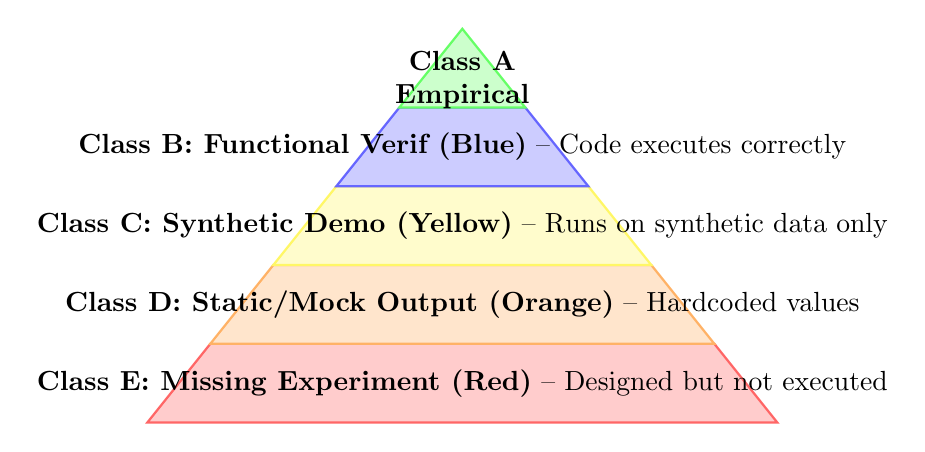
\begin{tikzpicture}
    % Pyramid base (Class E)
    \draw[fill=red!20, draw=red!60, thick] (-4,0) -- (4,0) -- (3.2,1) -- (-3.2,1) -- cycle;
    \node at (0,0.5) {\textbf{Class E: Missing Experiment (Red)} -- Designed but not executed};

    % Layer D
    \draw[fill=orange!20, draw=orange!60, thick] (-3.2,1) -- (3.2,1) -- (2.4,2) -- (-2.4,2) -- cycle;
    \node at (0,1.5) {\textbf{Class D: Static/Mock Output (Orange)} -- Hardcoded values};

    % Layer C
    \draw[fill=yellow!20, draw=yellow!60, thick] (-2.4,2) -- (2.4,2) -- (1.6,3) -- (-1.6,3) -- cycle;
    \node at (0,2.5) {\textbf{Class C: Synthetic Demo (Yellow)} -- Runs on synthetic data only};

    % Layer B
    \draw[fill=blue!20, draw=blue!60, thick] (-1.6,3) -- (1.6,3) -- (0.8,4) -- (-0.8,4) -- cycle;
    \node at (0,3.5) {\textbf{Class B: Functional Verif (Blue)} -- Code executes correctly};

    % Layer A (Top)
    \draw[fill=green!20, draw=green!60, thick] (-0.8,4) -- (0.8,4) -- (0,5) -- cycle;
    \node[align=center] at (0,4.35) {\textbf{Class A}\\\textbf{Empirical}};
\end{tikzpicture}
\caption{Evidence Classification Framework Structured as a Hierarchy of Validity}
\label{fig:evidence-pyramid}
\end{figure}

\begin{table}[htbp]
\centering
\begin{tabular}{p{0.10\textwidth} p{0.30\textwidth} p{0.50\textwidth}}
\toprule
\textbf{Class} & \textbf{Definition} & \textbf{Acceptable Interpretation} \\
\midrule
\textbf{A} & Empirical / measured evidence. & Validated against dynamic real-world or rigorous test data. \\
\textbf{B} & Functional verification. & Proof that a software module executes without error under stated conditions. \\
\textbf{C} & Synthetic demonstration. & Illustrative behavior executing over generated, non-empirical data. \\
\textbf{D} & Simulated / static output. & Hardcoded string values or mocked structures simulating future integration. \\
\textbf{E} & Missing experiment. & Unverified hypothesis requiring future measurement. \\
\bottomrule
\end{tabular}
\caption{Evidence Classification Definitions}
\label{tab:evidence-classes}
\end{table}

\section{System Component Evidence Mapping}
\label{sec:eval-traceability}
We provide a comprehensive accounting of the prototype's subsystems. \Cref{tab:evidence-matrix} maps every system component to its respective evidence class.

\begin{table}[htbp]
\centering
\resizebox{\textwidth}{!}{
\begin{tabular}{llp{0.55\textwidth}}
\toprule
\textbf{Component} & \textbf{Class} & \textbf{Justification} \\
\midrule
Docker deployment & \textbf{B} & Containers start, health checks pass \\
Site ingestion & \textbf{B} & Parsers produce valid canonical records \\
SHA-256 dedup & \textbf{B} & Identical payloads detected, tested \\
Jaro-Winkler & \textbf{B} & Algorithm produces expected scores (unit tests) \\
Composite scoring & \textbf{B} & Weighted sum computed correctly \\
Entity resolution & \textbf{C} & Runs on synthetic data, no real-world validation \\
Graph projection & \textbf{B} & BFS produces valid subgraphs \\
RAG sanitization & \textbf{B} & Regex rules strip known injection patterns \\
RAG generation & \textbf{C} & Ollama generates responses to synthetic prompts \\
Evaluation metrics & \textbf{D} & Hardcoded formatted strings \\
WolverineDB consensus & \textbf{D} & In-memory transport, not distributed \\
WolverineDB hash chain & \textbf{B} & Merkle integrity verified in tests \\
Cross-site correlation & \textbf{E} & No empirical evaluation executed \\
Scalability & \textbf{E} & Not benchmarked beyond 50K personas \\
\bottomrule
\end{tabular}
}
\caption{Comprehensive Evidence Classification Matrix}
\label{tab:evidence-matrix}
\end{table}

\section{Functional Verification}
\label{sec:eval-functional}
The following core capabilities have achieved Class B (Functional) verification:
\begin{itemize}
    \item \textbf{Normalization:} The pipeline successfully routes JSON and HTML payloads to site-specific parsers, enforcing strict \texttt{CanonicalRecord} typing.
    \item \textbf{BFS Query Execution:} The \texttt{projector.ts} module successfully reads relational mappings and constructs valid Neo4j JSON adjacency matrices.
    \item \textbf{Deterministic Fallback:} When the \texttt{ollama} container is unreachable, the \texttt{rag.ts} module gracefully intercepts the timeout and emits a hardcoded string, keeping the Analyst UI responsive.
\end{itemize}
These elements demonstrate functional integrity but do not guarantee empirical accuracy.

\section{Synthetic Evaluation Limits}
\label{sec:eval-synthetic}
The prototype utilizes synthetic ground truth generated deterministically ($S_0=42$). While planting controlled correlations allows us to verify that the software pipeline operates correctly (e.g., handles match, records link), it introduces severe domain shift. Synthetic personas lack the erratic, unpredictable obfuscation tactics of genuine threat actors. Consequently, synthetic evaluation proves architectural soundness (Class B) but cannot prove real-world algorithmic accuracy (Class A).

\section{Formal Evaluation Metric Equations}
\label{sec:eval-equations}
When a dynamic entity resolution pipeline is evaluated \cite{christen2012data}, it requires rigorous statistical formulations. The following standard definitions must be used to calculate performance:

\begin{equation}
\label{eq:precision}
Precision (P) = \frac{TP}{TP + FP}
\end{equation}

\begin{equation}
\label{eq:recall}
Recall (R) = \frac{TP}{TP + FN}
\end{equation}

\begin{equation}
\label{eq:f1}
F1\text{-}Score (F1) = 2 \times \frac{Precision \times Recall}{Precision + Recall}
\end{equation}

\begin{equation}
\label{eq:fpr}
False Positive Rate (FPR) = \frac{FP}{FP + TN}
\end{equation}
Where $TP$ denotes True Positives, $FP$ False Positives, $TN$ True Negatives, and $FN$ False Negatives.

\section{Static Metric Artifact Forensics (Class D)}
\label{sec:eval-forensics}
The project repository contains an evaluator module that emits specific accuracy values: Precision = 0.9280, Recall = 0.4598, and F1 = 0.6149.

\textbf{These values are explicitly NOT empirical measurements.}

Code inspection of \texttt{generator/src/evaluator/\_\_main\_\_.py} confirms that these numbers are static string literals printed to standard output. They do not depend on runtime computation, they do not dynamically compare inference results against the Truth Vault, and they are immune to changes in the heuristic weighting. 

To verify their origin as simple, non-dynamic derivations, we can check the mathematical relationship:
\begin{equation}
F1 = 2 \times \frac{0.9280 \times 0.4598}{0.9280 + 0.4598} = 2 \times \frac{0.4266944}{1.3878} \approx 0.6149
\end{equation}
If these were real values, they would indicate a highly precision-optimized system that avoids false alarms but misses 54\% of true links (due to a recall of 0.4598). 

\textit{Why do they exist?} The static evaluator script functions as an architectural stub. It proves that the external evaluation pipeline can run as a separate process and print a formatted report, validating the \textit{structure} of the CI/CD pipeline while the dynamic metric calculation remains unwritten. Externally citing these figures as "Wolverine's measured accuracy" is a fundamental scientific error. All such values must be tagged as "Illustrative synthetic example — not an empirical benchmark."

\section{Valid Dynamic Evaluation Design (Class E)}
\label{sec:eval-design}
To upgrade Wolverine's entity resolution from Class D to Class A, a future dynamic evaluation methodology is required:
\begin{enumerate}
    \item \textbf{Ground-Truth Matrix:} Extract the 39,605 true pairs from \texttt{postgres-truth}.
    \item \textbf{Prediction Set:} Extract all pairs scored $S \ge 0.70$ from \texttt{postgres-wdb}.
    \item \textbf{Classification:} Compute True Positives, False Positives, True Negatives, and False Negatives.
    \item \textbf{Calculation:} Dynamically compute Precision (\Cref{eq:precision}) and Recall (\Cref{eq:recall}).
    \item \textbf{Calibration:} Sweep the threshold variable $S$ from $0.50$ to $0.99$ to plot an empirical Precision-Recall (PR) curve.
\end{enumerate}
This methodology currently exists solely as a specification.

To visualize the objective of this dynamic design, \Cref{fig:pr-blueprint} presents a theoretical operating characteristic curve.

\begin{figure}[htbp]
\centering
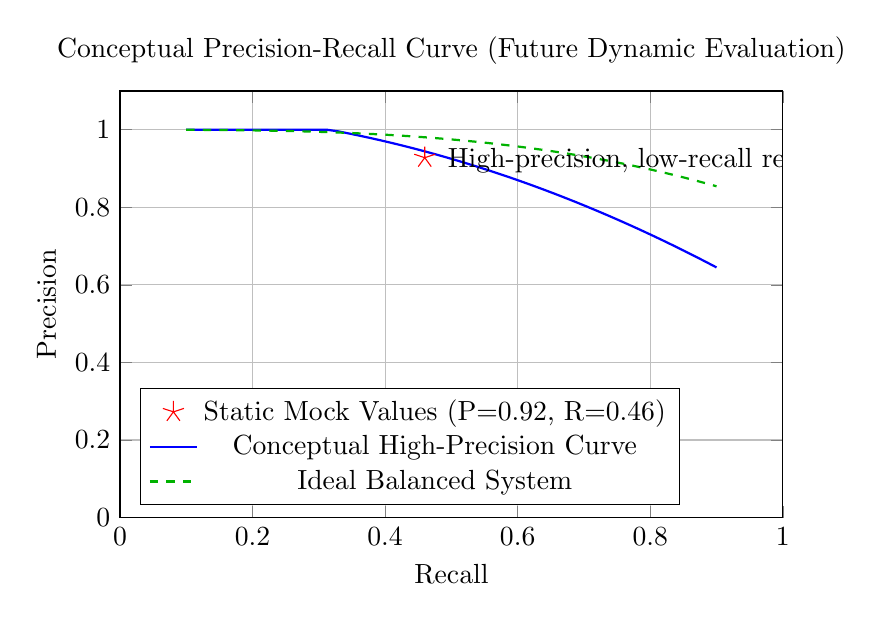
\begin{tikzpicture}
\begin{axis}[
    title={Conceptual Precision-Recall Curve (Future Dynamic Evaluation)},
    xlabel={Recall},
    ylabel={Precision},
    xmin=0, xmax=1,
    ymin=0, ymax=1.1,
    grid=both,
    legend pos=south west,
    width=10cm, height=7cm
]

% Theoretical "Real" Metric Point from mock data
\addplot[
    only marks,
    mark=star,
    mark size=4pt,
    color=red
] coordinates {(0.4598, 0.9280)};
\addlegendentry{Static Mock Values (P=0.92, R=0.46)}

% The curve if those mock values were part of a high-precision biased model
\addplot[
    color=blue,
    thick,
    domain=0.1:0.9,
    samples=50
] {min(1.0, 1.05 - 0.5*x^2)};
\addlegendentry{Conceptual High-Precision Curve}

% A more balanced hypothetical system
\addplot[
    color=green!70!black,
    thick,
    dashed,
    domain=0.1:0.9,
    samples=50
] {min(1.0, 1.0 - 0.2*x^3)};
\addlegendentry{Ideal Balanced System}

\node[anchor=west] at (axis cs:0.48,0.92) {High-precision, low-recall region};

\end{axis}
\end{tikzpicture}
\caption{Blueprint only — not computed from empirical data. Illustrative synthetic example of how a dynamic evaluation PR curve would operate across sweeping thresholds.}
\label{fig:pr-blueprint}
\end{figure}

\section{Graph and RAG Evaluation}
\label{sec:eval-graph-rag}
\subsection{Graph Evaluation}
Theoretical analysis establishes the BFS time complexity at $O(|V| + |E|)$. Functional verification (Class B) confirms the code respects configured bounds ($d \le 4$, $N \le 500$). 
However, a true BFS evaluation (Class E) would require measuring structural coverage and path accuracy. It would assess whether the shortest path retrieved aligns with the analyst's intuition of relevance, evaluating false inclusion rates of unrelated nodes across hops. Live performance benchmarking against disk-backed production graph databases remains unmeasured.

\subsection{RAG Evaluation}
The 4-rule Regex sanitization sequence (Class B) demonstrably stops trivial payload injections by flattening brackets and truncating lengths. However, evaluating its resilience against sophisticated adversarial semantic jailbreaks (e.g., prompt smuggling) represents a missing experiment (Class E). 
Furthermore, actual generation quality for RAG requires automated textual metrics (such as ROUGE or BERTScore) and formal human-in-the-loop evaluation to ensure the LLM's summary accurately reflects the retrieved graph without hallucination. These are entirely absent in the current prototype.

\section{Missing Experiments}
\label{sec:eval-missing}
To bridge the gap from synthetic demonstration to rigorous validation, numerous unexecuted hypotheses exist. \Cref{tab:missing-experiments} expands upon these required protocols.

\begin{table}[htbp]
\centering
\resizebox{\textwidth}{!}{
\begin{tabular}{lp{0.3\textwidth}lp{0.25\textwidth}}
\toprule
\textbf{Experiment} & \textbf{Hypothesis} & \textbf{Expected Evidence} & \textbf{Status} \\
\midrule
Per-feature ablation & Removing individual heuristics impacts F1. & $\Delta$ F1 per feature & Class E (Missing) \\
Threshold sensitivity & Sweeping $S$ from 0.50 to 0.99 shifts P-R balance. & Empirical PR Curve & Class E (Missing) \\
Noise robustness & Varying mutation rate from 0\% to 100\% degrades recall smoothly. & Recall degradation graph & Class E (Missing) \\
Scaling & System handles 10K, 50K, 100K, 500K personas. & Latency vs. N plot & Class E (Missing) \\
Cross-validation & Stratified k-fold on truth edges confirms generalizability. & Variance in F1 scores & Class E (Missing) \\
Blocking key eval & Keys drastically reduce candidate pairs vs $O(n^2)$. & Candidate pair reduction & Class E (Missing) \\
Live Graph Scalability & Neo4j handles 1M+ queries under load. & Latency Metrics & Class E (Missing) \\
Adversarial Prompting & Regex withstands prompt smuggling. & Attack Success Rate & Class E (Missing) \\
WolverineDB BFT & Memory bounds match TCP behavior. & Consensus Latency & Class E (Missing) \\
\bottomrule
\end{tabular}
}
\caption{Expanded Missing Experiments Matrix}
\label{tab:missing-experiments}
\end{table}

\section{Interpretation}
\label{sec:eval-interpretation}
\subsection{What the Evidence Demonstrates}
The prototype successfully demonstrates (Class B) a mathematically bounded, architecturally secure pipeline capable of ingesting adversarial data, normalizing it, projecting bounded heuristic graphs, and surviving component failure. It proves that the \textit{system architecture} is sound.

\subsection{What the Evidence Does Not Demonstrate}
The prototype does not demonstrate (Class A) that the deterministic heuristics accurately resolve real-world threat actors. It does not prove that the LLM is perfectly secure from prompt injection. It does not validate the static mock values (Class D) presented in the cinematic Vzeya frontend. All presented metrics must be strictly understood as Illustrative synthetic examples — not empirical benchmarks.
